\documentclass[11pt]{article}

\usepackage[margin=1in]{geometry}
\usepackage{graphicx}
\usepackage{booktabs}
\usepackage{array}
\usepackage{longtable}
\usepackage{float}
\usepackage{caption}
\usepackage{amsmath}
\usepackage{enumitem}
\usepackage{url}
\usepackage[hidelinks]{hyperref}

\setlist[itemize]{leftmargin=1.4em}
\setlist[enumerate]{leftmargin=1.6em}
\captionsetup{font=small,labelfont=bf}

\title{Early Report: MLSS Exoplanet Habitability Classifier}
\author{Bhargav Dave}
\date{\today}

\begin{document}

\maketitle

\begin{abstract}
This report documents the current state of an MLSS course project that builds a binary classifier for exoplanet habitability labels. The current project is notebook-first and uses a Kepler Object of Interest (KOI) cumulative exoplanet dataset together with separate habitable and non-habitable planet lists. The report explains the data construction, selected feature space, exploratory analysis, preprocessing, model families, and visible results saved in the notebook. It is intentionally explanatory rather than a new modeling stage: no raw data is included, no notebook cells are rerun, and no model results are regenerated. The main interpretive caution is that the target variable \texttt{habitable?} is derived from pre-existing labeled lists, so high predictive scores indicate successful reproduction of that label distinction rather than definitive proof of physical or biological habitability.
\end{abstract}

\tableofcontents
\newpage

\section{Project Overview}

This report explains the current state of the MLSS exoplanet classifier notebook. The project is a graduate-level data science and machine learning course project focused on binary classification: predicting whether an exoplanet candidate is labeled habitable or non-habitable.

The current notebook is preserved as a historical course artifact at:

\begin{center}
\texttt{notebooks/mlss-dacss756-final-project-bdave\_v10.ipynb}
\end{center}

The notebook title currently reads ``Predicting the Hability of Exoplanets using Machine Learning.'' The word ``Hability'' should eventually be corrected to ``Habitability,'' but the notebook itself has not been edited for this report.

The modeling goal is to learn a relationship between selected KOI numeric features and a binary target variable called \texttt{habitable?}. A value of 1 represents planets from a habitable list, and a value of 0 represents planets from a non-habitable list. This is a supervised classification problem, not an unsupervised discovery task.

\section{Dataset and Provenance}

The notebook describes the data as Kepler exoplanet and KOI data. It loads a cumulative KOI-style dataset plus two separate labeled files:

\begin{itemize}
  \item \texttt{cumulative-exoplanets.xlsx}
  \item \texttt{habitable\_planets\_detailed\_list.xlsx}
  \item \texttt{non\_habitable\_planets\_confirmed\_detailed\_list.xlsx}
\end{itemize}

The raw data files are not included in the clean GitHub repository or in this Overleaf package. This report uses only saved notebook outputs and existing report artifacts.

The visible notebook output shows that the original cumulative table contains 9,564 rows and 141 columns. The notebook keeps only a subset of columns for modeling: \texttt{kepoi\_name}, 15 numeric KOI features, and later the target variable \texttt{habitable?}.

The NASA Exoplanet Archive documentation for the Kepler Object of Interest table describes KOI columns returned through the Exoplanet Archive API, including identifiers and physical/orbital columns such as KOI name, orbital period, planet radius, and stellar parameters \cite{nasaKoiColumns}. This report does not overclaim provenance beyond what the notebook shows: the notebook uses Kaggle-style input paths and describes the underlying data as Kepler/KOI data.

\section{Target Construction}

The target variable is \texttt{habitable?}. The notebook constructs it in three steps:

\begin{enumerate}
  \item Assign \texttt{habitable? = 1} to every row in the habitable planet list.
  \item Assign \texttt{habitable? = 0} to every row in the non-habitable confirmed planet list.
  \item Concatenate those label tables and merge them onto the filtered KOI feature table by \texttt{kepoi\_name}.
\end{enumerate}

After this merge, the visible modeling dataset has 2,372 rows and 17 columns. Those columns consist of \texttt{kepoi\_name}, the 15 numeric modeling features, and \texttt{habitable?}.

This construction is central to interpretation. The model is learning to reproduce labels derived from pre-existing habitable and non-habitable lists. It is not directly measuring biological habitability, biosignatures, surface conditions, atmospheric composition, or life. A high score means the model separates these two label-list groups using selected KOI features. It does not prove that the model has discovered physical habitability in a broader scientific sense.

A related limitation is possible label-feature dependence. If the habitable and non-habitable lists were created using variables similar to the predictors, then the model may partly learn the same rules used to construct the labels. That can still be reasonable for a course classifier, but it should be documented carefully.

\section{Feature Space}

The notebook uses 15 numeric KOI-style features. These features mix planet-candidate properties, orbital geometry, and host-star properties. Table~\ref{tab:features} gives plain-language descriptions.

\begin{longtable}{>{\ttfamily}p{0.22\textwidth}p{0.70\textwidth}}
\caption{Selected modeling features and plain-language descriptions.}
\label{tab:features}\\
\toprule
\normalfont Feature & Description \\
\midrule
\endfirsthead
\toprule
\normalfont Feature & Description \\
\midrule
\endhead
koi\_period & Orbital period, usually measured in days. It describes how long the object takes to complete one orbit. \\
koi\_ror & Planet-star radius ratio. It compares the estimated radius of the planet candidate with the radius of its host star. \\
koi\_srho & Fitted stellar density. It is a stellar-density estimate associated with the transit model. \\
koi\_prad & Planetary radius in Earth radii. This is relevant because extremely large objects are less Earth-like. \\
koi\_sma & Semi-major axis in astronomical units. This approximates orbital scale or distance from the host star. \\
koi\_teq & Equilibrium temperature in Kelvin. This is an estimated temperature under simplifying assumptions, not a measured surface temperature. \\
koi\_insol & Insolation flux relative to Earth. It estimates how much stellar energy the planet receives. \\
koi\_dor & Planet-star distance divided by stellar radius. This is a scaled orbital-distance quantity. \\
koi\_count & Count of planets or KOIs associated with the system in the KOI table context. \\
koi\_steff & Stellar effective temperature in Kelvin. This describes the host star, not the planet itself. \\
koi\_slogg & Stellar surface gravity, typically in $\log_{10}(\mathrm{cm}/\mathrm{s}^2)$. This is a host-star property. \\
koi\_smet & Stellar metallicity in dex. This is a host-star composition-related estimate. \\
koi\_srad & Stellar radius in solar radii. This is the size of the host star relative to the Sun. \\
koi\_smass & Stellar mass in solar masses. This is the host-star mass relative to the Sun. \\
koi\_eccen & Orbital eccentricity. It describes how circular or elongated the orbit is. \\
\bottomrule
\end{longtable}

\section{Exploratory Data Analysis}

The notebook performs exploratory data analysis after merging labels onto the selected KOI features. The key visible row counts are:

\begin{itemize}
  \item Original cumulative dataset: 9,564 rows and 141 columns.
  \item Merged modeling dataset: 2,372 rows and 17 columns.
  \item Dataset after outlier removal: 2,121 rows.
\end{itemize}

Visible missingness before processing shows that \texttt{kepoi\_name}, \texttt{koi\_period}, \texttt{koi\_count}, and \texttt{habitable?} have 0 missing values, while many other numeric feature columns have 1 missing value each.

Figure~\ref{fig:eda-boxplots} shows the saved notebook boxplots for the 15 numeric features before outlier handling. Figure~\ref{fig:target-distribution} shows the target class distribution.

\begin{figure}[H]
  \centering
  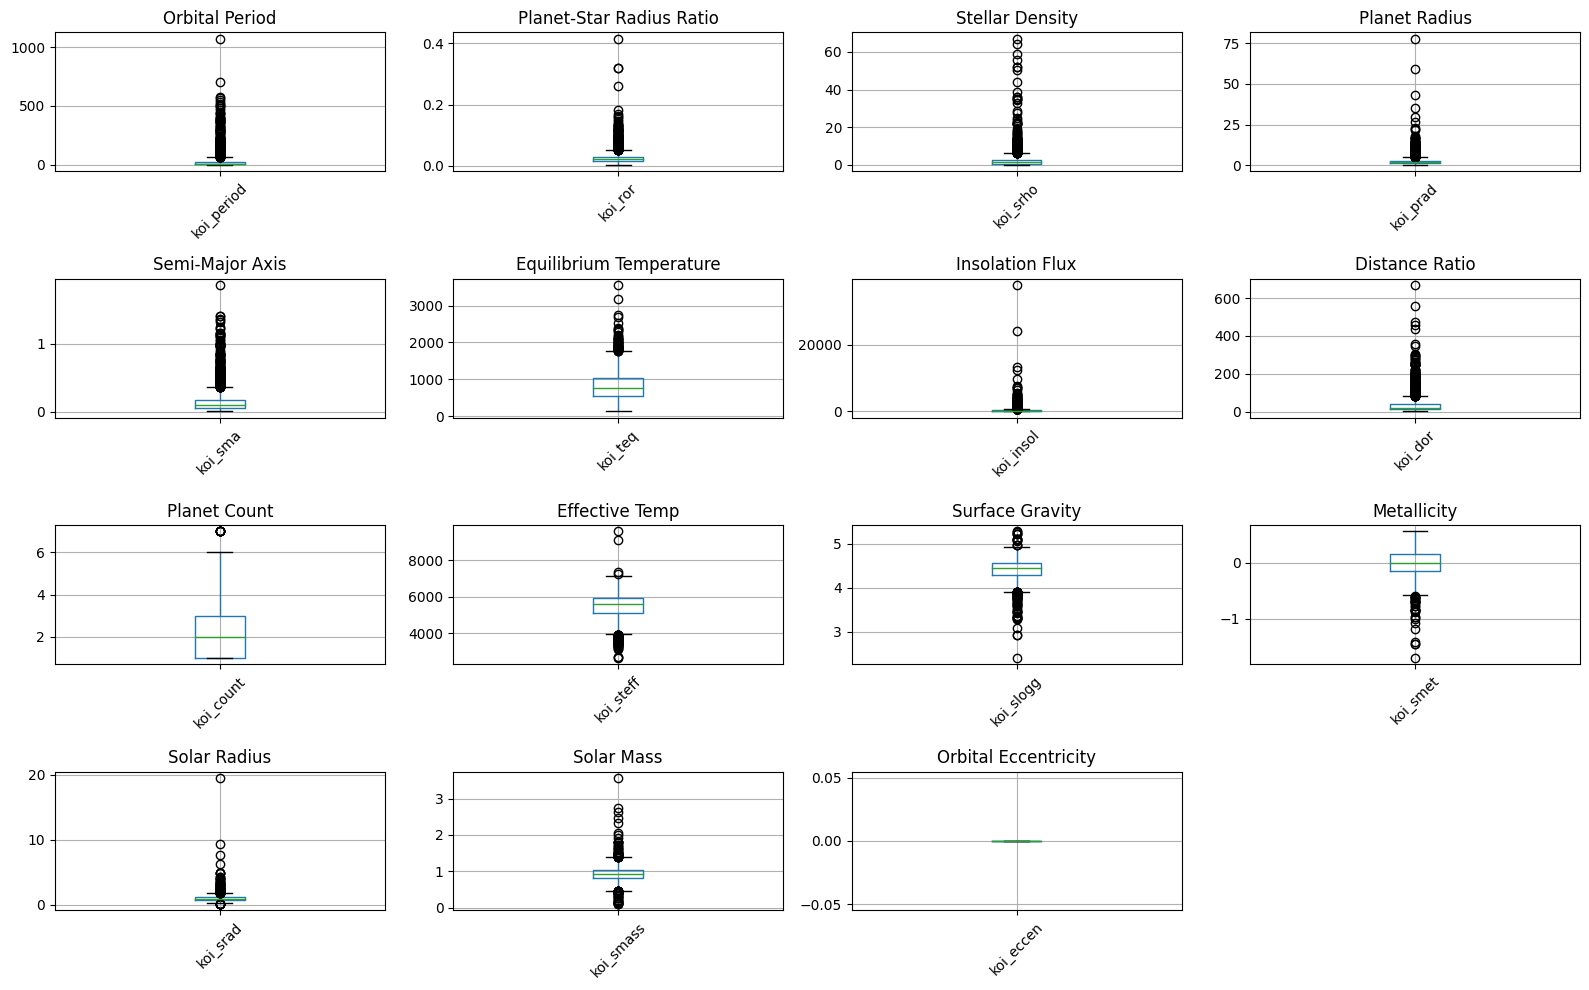
\includegraphics[width=\textwidth]{figures/01_feature_boxplots_before_outlier_removal.png}
  \caption{Feature boxplots before outlier removal. The saved notebook output shows substantial spread and potential outliers across several numeric KOI features.}
  \label{fig:eda-boxplots}
\end{figure}

\begin{figure}[H]
  \centering
  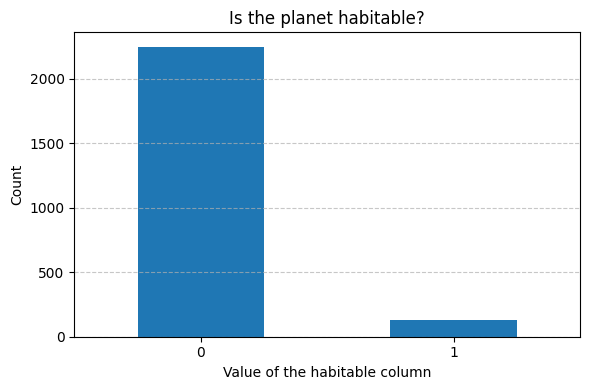
\includegraphics[width=0.70\textwidth]{figures/02_target_class_distribution.png}
  \caption{Target class distribution for \texttt{habitable?}. The visible notebook output indicates strong class imbalance.}
  \label{fig:target-distribution}
\end{figure}

The processed class distribution is highly imbalanced. The visible split sanity check reports approximately 94.86\% class 0 and 5.14\% class 1 overall. This imbalance explains why the notebook does not rely on accuracy alone.

\section{Outlier Handling}

The notebook defines an interquartile range (IQR) filtering function. For a chosen column,

\[
\mathrm{IQR} = Q_3 - Q_1,
\]

\[
\mathrm{lower\ bound} = Q_1 - \mathrm{multiplier} \times \mathrm{IQR},
\qquad
\mathrm{upper\ bound} = Q_3 + \mathrm{multiplier} \times \mathrm{IQR}.
\]

Rows outside the interval are removed. The notebook applies this filtering to two features:

\begin{itemize}
  \item \texttt{koi\_smass}, using IQR multiplier 1.5.
  \item \texttt{koi\_prad}, using IQR multiplier 2.
\end{itemize}

The visible row counts are:

\begin{itemize}
  \item Before \texttt{koi\_smass} filtering: 2,372 rows.
  \item After \texttt{koi\_smass} filtering: 2,276 rows.
  \item After \texttt{koi\_prad} filtering: 2,121 rows.
\end{itemize}

This choice should be documented carefully. Outlier removal can strongly affect rare classes, and the habitable class is only about 5\% of the processed data. Removing rows based on stellar mass or planet radius may remove physically unusual but scientifically meaningful cases. A future workflow should quantify whether filtering disproportionately removes class 1.

\section{Train-Test Split and Imputation}

The notebook separates features and target after outlier filtering:

\begin{itemize}
  \item \texttt{X}: the 15 numeric features.
  \item \texttt{y}: \texttt{habitable?}.
\end{itemize}

It then performs an 80/20 train-test split with \texttt{test\_size=0.2}, \texttt{stratify=y}, and \texttt{random\_state=42}. Stratification is important because the positive class is small. Without stratification, a random split could place too few habitable-class examples in either train or test.

The visible classification reports show the test set has 403 class 0 examples and 22 class 1 examples. That small positive-class test support is a major interpretation caveat: one or two changed predictions can noticeably affect positive-class precision, recall, and F1.

The notebook uses median imputation. It fits \texttt{SimpleImputer(strategy='median')} on \texttt{X\_train} and applies it to \texttt{X\_test}. This is better than fitting imputation before the split, because the test set does not influence the training-set medians.

However, future refactoring should move imputation inside scikit-learn \texttt{Pipeline} and, if needed, \texttt{ColumnTransformer} objects \cite{sklearnPipeline,sklearnColumnTransformer}. In the current notebook, imputation is fit before cross-validation over \texttt{X\_train}, which means median values are computed from the full training set before internal CV folds are made. Because missingness is tiny here, the practical effect may be small, but the leakage-safe pattern is to fit preprocessing inside each CV fold.

\begin{figure}[H]
  \centering
  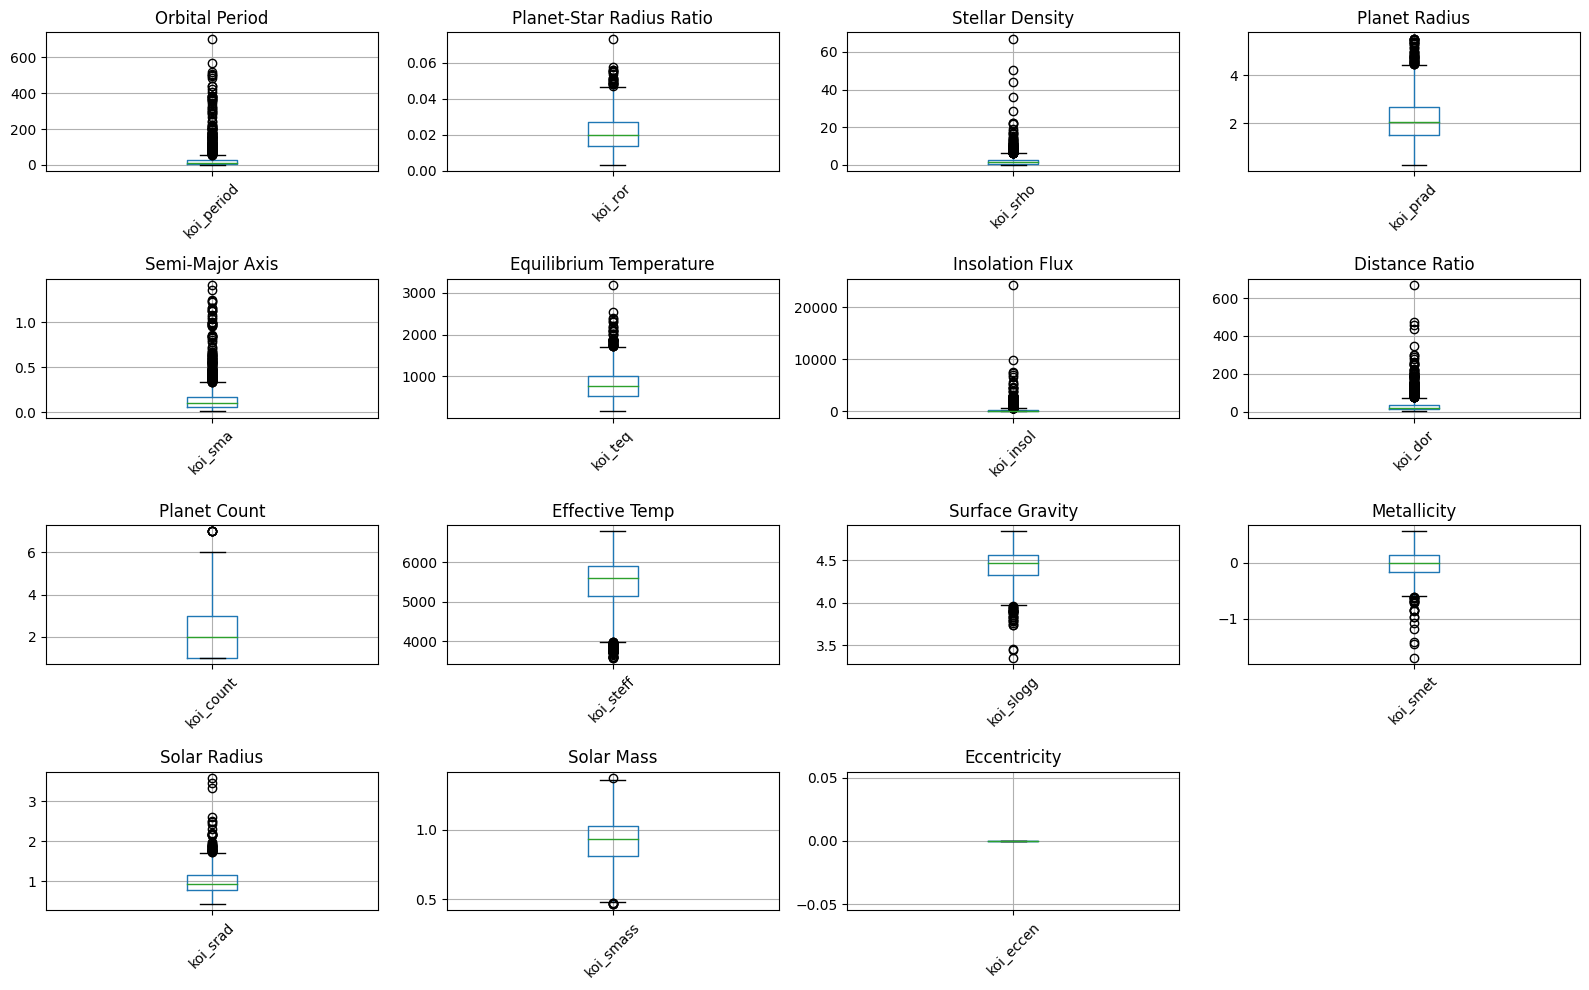
\includegraphics[width=\textwidth]{figures/03_training_feature_boxplots_after_split.png}
  \caption{Training feature boxplots after the train-test split, as saved in the notebook output.}
  \label{fig:training-boxplots}
\end{figure}

\section{Evaluation Metric}

The notebook uses macro F1 as the main model-selection metric. For binary classification:

\begin{itemize}
  \item Accuracy is the fraction of all predictions that are correct.
  \item Precision asks: among predicted positives, how many are truly positive?
  \item Recall asks: among actual positives, how many were found?
  \item F1 is the harmonic mean of precision and recall.
\end{itemize}

The scikit-learn documentation defines F1 as a balance between precision and recall \cite{sklearnF1Score}. F1 is useful when the positive class is important and class distribution is imbalanced.

Macro averaging computes the metric separately for each class, then averages the class-level values. This gives class 0 and class 1 equal weight, even though class 1 is much smaller. A classifier can achieve high accuracy by mostly predicting the majority class, but macro F1 penalizes poor minority-class performance.

The notebook uses \texttt{GridSearchCV} with 5-fold cross-validation and \texttt{scoring='f1\_macro'}. Cross-validation estimates model performance across multiple train/validation splits, and grid search tries parameter combinations to select the best setting under the chosen metric \cite{sklearnCrossValidation,sklearnGridSearchCV}.

\section{Logistic Regression Models}

Binary logistic regression models the probability that an example belongs to class 1 rather than class 0. It learns a linear decision boundary in the feature space. In this project, the inputs are numeric exoplanet and stellar features, and the output is the classification target \texttt{habitable?}.

Because logistic regression is sensitive to feature scale, the notebook uses \texttt{StandardScaler} inside scikit-learn pipelines for the logistic models. Scaling matters because features such as orbital period, stellar temperature, and metallicity exist on very different numeric ranges.

The notebook evaluates three regularized logistic regression variants:

\begin{itemize}
  \item L1 regularization, also called lasso-style regularization. It can push some coefficients toward exactly zero.
  \item L2 regularization, also called ridge-style regularization. It shrinks coefficients but usually does not set them exactly to zero.
  \item Elastic Net regularization, which combines L1 and L2 penalties.
\end{itemize}

The notebook searches over \texttt{C}, where \texttt{C} is the inverse of regularization strength. Smaller \texttt{C} means stronger regularization; larger \texttt{C} means weaker regularization.

Visible logistic regression results are:

\begin{itemize}
  \item L1 Logistic Regression: CV macro F1 = 0.9409.
  \item L2 Logistic Regression: CV macro F1 = 0.9384.
  \item Elastic Net Logistic Regression: CV macro F1 = 0.9419 and test macro F1 = 0.9648.
\end{itemize}

The final comparison table includes Elastic Net logistic regression, not the L1 and L2 variants. The Elastic Net model ties for the best visible test macro F1 in the final comparison.

\begin{figure}[H]
  \centering
  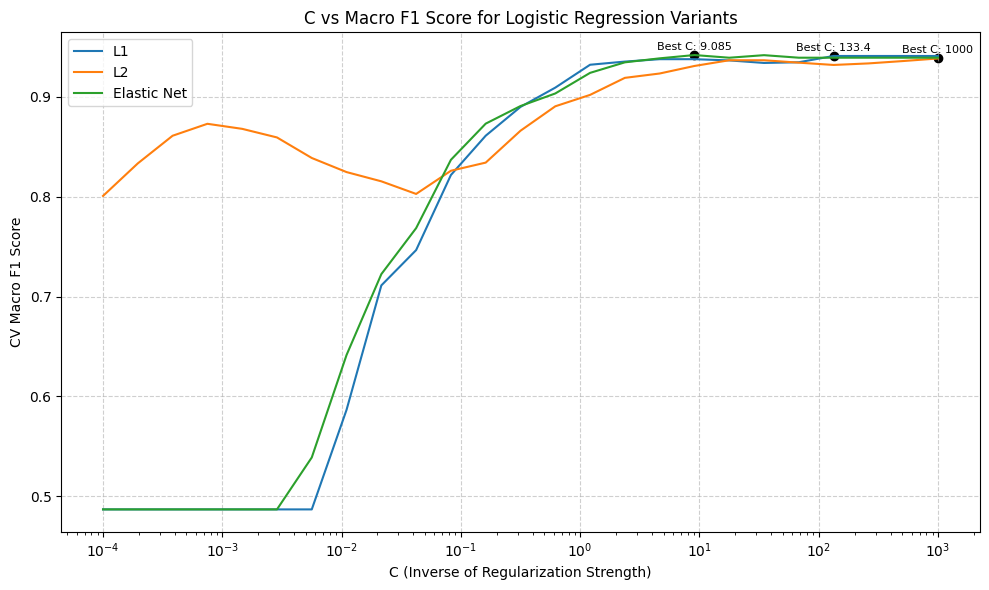
\includegraphics[width=0.82\textwidth]{figures/04_logistic_regression_cv_curve.png}
  \caption{Saved logistic regression cross-validation curve from the notebook.}
  \label{fig:logistic-cv}
\end{figure}

\section{Tree-Based Models}

Tree-based models split the feature space into regions using decision rules. A single decision tree can be intuitive, but it often overfits. Ensemble tree methods combine many trees to improve performance.

The notebook includes Random Forest, Gradient Boosting, and XGBoost.

\paragraph{Random Forest.}
Random Forest builds many decision trees and combines their predictions. It usually reduces variance relative to a single tree by using randomness in samples and/or selected features.

\paragraph{Gradient Boosting.}
Gradient Boosting builds trees sequentially. Each new tree attempts to improve the current ensemble by focusing on remaining errors.

\paragraph{XGBoost.}
XGBoost is an optimized gradient-boosting framework often used for tabular data. The original XGBoost paper describes it as a scalable tree boosting system \cite{chenGuestrin2016XGBoost}, and the official documentation describes the boosted-tree model formulation \cite{xgboostDocs}.

Visible tree-based results are:

\begin{itemize}
  \item Random Forest: CV macro F1 = 0.9718 and test macro F1 = 0.9540.
  \item Gradient Boosting / ``Random Forest With GBM'': CV macro F1 = 0.9720 and test macro F1 = 0.9540.
  \item XGBoost: CV macro F1 = 0.9647 and test macro F1 = 0.9413.
\end{itemize}

The notebook includes impurity-based feature importance plots. It reports \texttt{koi\_teq} as the most important Random Forest feature and \texttt{koi\_insol} as the most important Gradient Boosting feature.

\begin{figure}[H]
  \centering
  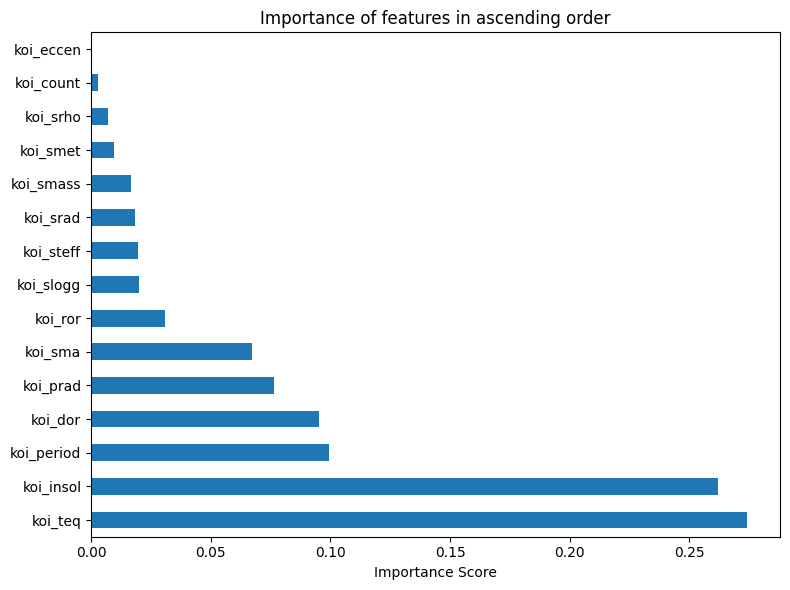
\includegraphics[width=0.78\textwidth]{figures/05_random_forest_feature_importance.png}
  \caption{Random Forest feature importance from the saved notebook output. The visible text identifies \texttt{koi\_teq} as the most important feature.}
  \label{fig:rf-importance}
\end{figure}

\begin{figure}[H]
  \centering
  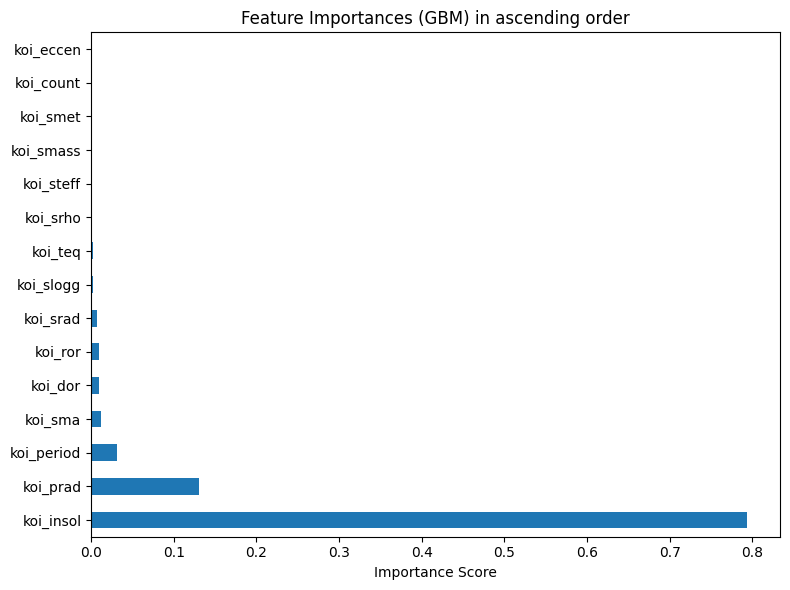
\includegraphics[width=0.78\textwidth]{figures/06_gradient_boosting_feature_importance.png}
  \caption{Gradient Boosting feature importance from the saved notebook output. The visible text identifies \texttt{koi\_insol} as the most important feature.}
  \label{fig:gbm-importance}
\end{figure}

These importances should be interpreted cautiously. Impurity-based feature importance can favor variables with certain distributions or many possible split points, and correlated features can share or distort importance. Future work should add permutation importance as a more model-agnostic check.

\section{Support Vector Machines}

Support vector machines classify examples by finding a boundary that separates classes with a large margin. The support vectors are the training points closest to the decision boundary; they help define the margin.

The notebook evaluates three SVM kernels:

\begin{itemize}
  \item Linear kernel: learns a linear boundary.
  \item Polynomial kernel: allows curved boundaries based on polynomial feature interactions.
  \item RBF kernel: allows flexible nonlinear boundaries based on radial similarity.
\end{itemize}

The key hyperparameters include:

\begin{itemize}
  \item \texttt{C}: controls the tradeoff between margin size and training errors.
  \item \texttt{gamma}: controls locality of influence for kernels such as RBF.
  \item \texttt{degree}: controls polynomial complexity for the polynomial kernel.
\end{itemize}

The notebook uses \texttt{StandardScaler} for SVM models because SVM distances and margins depend on feature magnitude.

Visible SVM results are:

\begin{itemize}
  \item SVM Linear: CV macro F1 = 0.9419 and test macro F1 = 0.9540.
  \item SVM Polynomial: CV macro F1 = 0.9399 and test macro F1 = 0.9338.
  \item SVM RBF: CV macro F1 = 0.9421 and test macro F1 = 0.9648.
\end{itemize}

The RBF SVM ties Elastic Net logistic regression for the best visible test macro F1 in the final comparison.

\section{Model Comparison}

Table~\ref{tab:model-comparison} reproduces the final visible model comparison table. These values are also stored in the report package under \texttt{tables/model\_comparison.csv} and \texttt{tables/model\_comparison.md}.

\begin{table}[H]
\centering
\caption{Visible final model comparison from the notebook.}
\label{tab:model-comparison}
\small
\begin{tabular}{lcc}
\toprule
Model & CV macro F1 & Test macro F1 \\
\midrule
Logistic Regression (Elastic Net) & 0.9419 & 0.9648 \\
Random Forest & 0.9718 & 0.9540 \\
Gradient Boosting / ``Random Forest With GBM'' & 0.9720 & 0.9540 \\
XGBoost & 0.9647 & 0.9413 \\
SVM Linear & 0.9419 & 0.9540 \\
SVM Polynomial & 0.9399 & 0.9338 \\
SVM RBF & 0.9421 & 0.9648 \\
\bottomrule
\end{tabular}
\end{table}

The notebook label ``Random Forest With GBM'' appears to refer to the Gradient Boosting model implemented with \texttt{GradientBoostingClassifier}. This report uses the combined label ``Gradient Boosting / Random Forest With GBM'' to preserve the visible notebook wording while clarifying the method.

\section{Interpretation of Results}

The best visible test macro F1 values are:

\begin{itemize}
  \item Logistic Regression Elastic Net: 0.9648.
  \item SVM RBF: 0.9648.
\end{itemize}

The best visible cross-validated macro F1 values are:

\begin{itemize}
  \item Gradient Boosting: 0.9720.
  \item Random Forest: 0.9718.
\end{itemize}

This creates a useful interpretation question. The tree-based models have stronger CV macro F1 scores, but Elastic Net logistic regression and RBF SVM have the highest visible test macro F1. That does not automatically mean the latter are truly better in general. The test set contains only 22 habitable-class cases, so the test macro F1 estimate for class 1 is high-variance. With such small positive test support, a small number of changed predictions can materially alter the result.

The repeated use of the same test set for final model reporting should also be interpreted with care. That is common in course notebooks, but if modeling decisions are influenced by test results, the test set starts to behave like part of the model-selection loop. A stronger future workflow would preserve a final holdout set or use nested cross-validation if rigorous model-selection claims are required.

High scores may indicate that the selected KOI features strongly reproduce the distinction in the pre-labeled habitable and non-habitable lists. That is a valid supervised-learning result, but it should not be stated as proof of definitive physical habitability. The model is learning labels, and the meaning of those labels depends on how the label files were originally constructed.

\section{Limitations}

The current project has several limitations that should be acknowledged.

\begin{itemize}
  \item The target is derived from two pre-labeled files and is not a direct biological habitability measurement.
  \item The processed data is about 94.86\% class 0 and 5.14\% class 1.
  \item The visible test set has only 22 class 1 examples.
  \item If the label lists were created using features related to \texttt{koi\_teq}, \texttt{koi\_insol}, \texttt{koi\_prad}, or similar variables, the model may learn label-generation logic rather than independent habitability evidence.
  \item Imputation is fit after the train-test split, which is good, but it should be inside pipelines for cross-validation safety.
  \item Outlier filtering happens before train-test split and before imputation, so future work should document how it affects class balance.
  \item The notebook uses Kaggle-specific paths such as \texttt{/kaggle/input/...}.
  \item Raw data acquisition is not scripted.
  \item There is no root README yet.
  \item There is no requirements file yet.
  \item There are no automated tests yet.
  \item The workflow is notebook-only and not yet modular.
  \item The title typo ``Hability'' should eventually be corrected to ``Habitability.''
  \item Some labels should be standardized, such as ``Random Forest With GBM'' versus ``Gradient Boosting.''
\end{itemize}

\section{Roadmap for Improvement}

The enhanced version should preserve the original notebook as a course artifact, then build a clean reproducible workflow around it. Recommended improvements include:

\begin{itemize}
  \item Add a root README explaining the project goal, setup, data access, reproducible commands, and scientific caveats.
  \item Add \texttt{requirements.txt} or \texttt{pyproject.toml}.
  \item Add local path handling so the project does not depend on Kaggle-only paths.
  \item Add a config-driven workflow for paths, feature lists, split settings, model grids, and output locations.
  \item Move preprocessing into scikit-learn \texttt{Pipeline} and \texttt{ColumnTransformer} objects.
  \item Keep imputation, scaling, and model fitting leakage-safe inside cross-validation.
  \item Add a \texttt{DummyClassifier} baseline.
  \item Use bounded \texttt{GridSearchCV} or \texttt{RandomizedSearchCV} so searches are reproducible and not unnecessarily expensive.
  \item Reproduce existing notebook models before introducing any new modeling methods.
  \item Save model comparison artifacts as CSV, Markdown, and figures.
  \item Add confusion matrices, ROC curves, and precision-recall curves.
  \item Add permutation importance for model interpretation.
  \item Create a scientific caveats document explaining what the \texttt{habitable?} label does and does not mean.
  \item Add lightweight tests for schema expectations, feature selection, target construction, split stratification, and output creation.
  \item Add CLI scripts for data preparation, training, and evaluation.
  \item Define an optional model persistence policy, keeping model binaries out of Git.
\end{itemize}

The immediate next engineering stage should be reproducibility and structure, not new modeling complexity.

\newpage
\bibliographystyle{plain}
\bibliography{references}

\end{document}
